\documentclass[10pt,a4paper]{article}

\usepackage[utf8]{inputenc}
\usepackage[T1]{fontenc}
\usepackage{lmodern}
\usepackage[a4paper,top=1.8cm,bottom=1.8cm,left=1.8cm,right=1.8cm]{geometry}
\usepackage{xcolor}
\usepackage{tikz}
\usetikzlibrary{calc,shapes.geometric,backgrounds}
\usepackage{booktabs}
\usepackage{tabularx}
\usepackage{enumitem}
\usepackage{titlesec}
\usepackage{fancyhdr}
\usepackage{microtype}
\usepackage[colorlinks=true,linkcolor=primary,urlcolor=secondary]{hyperref}

% =========================================================
% Color Palette
% =========================================================
\definecolor{primary}{RGB}{30, 58, 138}        % Deep navy blue
\definecolor{secondary}{RGB}{2, 132, 199}      % Cyan/Sky blue
\definecolor{darkslate}{RGB}{51, 65, 85}       % Slate grey
\definecolor{bordergray}{RGB}{209, 213, 219}   % Light grey border
\definecolor{boxbg}{RGB}{248, 250, 252}        % Light subtle card bg

% Terminal Colors (Light Grey Theme)
\definecolor{termbg}{RGB}{246, 248, 250}       % Light grey background
\definecolor{termbar}{RGB}{229, 231, 235}      % Slightly darker grey title bar
\definecolor{termborder}{RGB}{209, 213, 219}   % Border grey
\definecolor{termtext}{RGB}{31, 41, 55}        % Dark charcoal text
\definecolor{termuser}{RGB}{22, 101, 52}       % Dark green for user
\definecolor{termhost}{RGB}{21, 128, 61}       % Green for host
\definecolor{termpath}{RGB}{29, 78, 216}       % Blue for directory path
\definecolor{termcmd}{RGB}{17, 24, 39}         % Bold black for commands
\definecolor{termout}{RGB}{55, 65, 81}         % Clear dark grey for outputs
\definecolor{termdir}{RGB}{37, 99, 235}        % Blue for directories
\definecolor{termfile}{RGB}{31, 41, 55}        % Dark for regular files
\definecolor{termhidden}{RGB}{107, 114, 128}   % Muted grey for hidden files
\definecolor{termsize}{RGB}{180, 83, 9}        % Amber for sizes
\definecolor{termperm}{RGB}{79, 70, 229}       % Indigo for permissions

% =========================================================
% Section Headings (Clean, No Underline)
% =========================================================
\titleformat{\section}
  {\color{primary}\large\bfseries\sffamily}
  {\thesection.}{0.5em}{}
\titlespacing*{\section}{0pt}{8pt}{3pt}

\titleformat{\subsection}
  {\color{secondary}\normalsize\bfseries\sffamily}
  {\thesubsection}{0.5em}{}
\titlespacing*{\subsection}{0pt}{6pt}{2pt}

% =========================================================
% Headers and Footers (Completely Clean Footers)
% =========================================================
\pagestyle{fancy}
\fancyhf{}
\renewcommand{\headrulewidth}{0.4pt}
\renewcommand{\footrulewidth}{0pt}
\fancyhead[L]{\small\sffamily\color{darkslate} Operating Systems Lab}
\fancyhead[R]{\small\sffamily\color{darkslate} Lab Report: Helpful Terminal Utilities}
\fancyfoot{}

% First page style: no header at top, no footer at bottom
\fancypagestyle{firstpage}{%
  \fancyhf{}
  \renewcommand{\headrulewidth}{0pt}
  \renewcommand{\footrulewidth}{0pt}
}

% =========================================================
% Terminal Window Macro (Light Grey with Crisp Edges)
% =========================================================
\newcommand{\termprompt}[1][\textasciitilde]{%
  \textbf{\textcolor{termuser}{ratul}}\textcolor{termtext}{@}\textbf{\textcolor{termhost}{firefly}}\textcolor{termtext}{:}\textbf{\textcolor{termpath}{#1}}\textcolor{termcmd}{\$}\ %
}

\newcommand{\terminalwindow}[3][\linewidth]{%
\begin{center}
\begin{tikzpicture}
  % 1. Terminal text on main layer
  \node[
      text=termtext,
      font=\ttfamily\fontsize{7.2}{9.2}\selectfont,
      align=left,
      text width=\dimexpr#1-0.95cm\relax,
      inner xsep=7pt,
      inner ysep=7pt,
      anchor=north west
  ] (body) at (0.32cm, -0.56cm) {#3};

  % Coordinates
  \coordinate (topleft) at (0, 0);
  \coordinate (bottomright) at ($(body.south -| #1, 0) + (0, -6pt)$);
  \coordinate (titlecenter) at ($0.5*(topleft) + 0.5*(#1, 0) + (0, -0.28cm)$);

  % 2. Background and Title bar on background layer
  \begin{scope}[on background layer]
    % Light grey terminal body
    \fill[termbg, rounded corners=6pt] (topleft) rectangle (bottomright);

    % Title bar (clipped to match rounded top corners)
    \begin{scope}
      \clip[rounded corners=6pt] (topleft) rectangle (bottomright);
      \fill[termbar] (topleft) rectangle (#1, -0.56cm);
      \draw[termborder, line width=0.5pt] (0, -0.56cm) -- (#1, -0.56cm);
    \end{scope}

    % Continuous outer border (smooth, no distortion)
    \draw[termborder, line width=0.6pt, rounded corners=6pt] (topleft) rectangle (bottomright);
  \end{scope}

  % 3. Window control dots
  \fill[red!80!black] (0.36cm, -0.28cm) circle (0.07cm);
  \fill[yellow!80!black] (0.63cm, -0.28cm) circle (0.07cm);
  \fill[green!75!black] (0.90cm, -0.28cm) circle (0.07cm);

  % 4. Centered terminal title
  \node[
      text=gray!40!black,
      font=\sffamily\bfseries\fontsize{7.2}{8}\selectfont,
      anchor=center
  ] at (titlecenter) {#2};
\end{tikzpicture}
\end{center}
\vspace{-6pt}
}

\newcommand{\cmd}[1]{\texttt{\textbf{#1}}}

\begin{document}
\thispagestyle{firstpage}

% =========================================================
% Title: Only Experiment Title at the Top
% =========================================================
\begin{center}
  {\Large\bfseries\sffamily\color{primary} Experiment Title: Helpful Utilities in Linux Terminal}\\[3pt]
  {\normalsize\sffamily\textbf{Topic:} Practical Everyday Utilities for Terminal Management, System Info, and Environment}
\end{center}
\vspace{-4pt}

% =========================================================
% 1. Objective
% =========================================================
\section{Objective}
The objective of this lab is to explore essential command-line utility tools that improve daily productivity and system awareness in Linux. By completing this experiment, we aim to:
\begin{itemize}[noitemsep,topsep=1pt,leftmargin=1.2em]
  \item Inspect user session and hardware names using \cmd{whoami}, \cmd{who}, and \cmd{hostname}.
  \item Display formatted messages, timestamps, and insert controlled pauses with \cmd{echo}, \cmd{date}, and \cmd{sleep}.
  \item Clean terminal clutter using \cmd{clear} and read built-in manual documentation using \cmd{man}.
  \item Review and recall past executed commands using \cmd{history}.
  \item Create custom command shortcuts using \cmd{alias} and inspect system environment variables with \cmd{env} and \cmd{printenv}.
\end{itemize}

% =========================================================
% 2. Equipment / Software Requirements
% =========================================================
\section{Equipment / Software Requirements}
\vspace{-2pt}
\begin{table}[h!]
\centering\footnotesize
\renewcommand{\arraystretch}{1.08}
\begin{tabularx}{\linewidth}{lXlX}
\toprule
\textbf{Item} & \textbf{Details} & \textbf{Item} & \textbf{Details} \\
\midrule
\textbf{Operating System} & Linux (NixOS 26.11 / Ubuntu 24.04) & \textbf{Host Machine} & \texttt{firefly} \\
\textbf{User Account} & \texttt{ratul} & \textbf{Command Shell} & GNU Bash 5.2 \\
\textbf{Terminal Emulator} & Linux Terminal (Kitty / Ghostty) & \textbf{Core Utilities} & GNU Coreutils, Bash Builtins, Man-db \\
\bottomrule
\end{tabularx}
\end{table}
\vspace{-8pt}

% =========================================================
% 3. Theoretical Background
% =========================================================
\section{Theoretical Background}
Linux provides a rich set of built-in helpers and utility programs. These tools don't just manipulate files; they reveal system identity, keep track of our workflow history, create personalized shortcuts, and allow scripts to pause and read system environment variables.

\subsection{Commands Practiced in This Lab}
\vspace{-2pt}
\begin{table}[h!]
\centering\footnotesize
\renewcommand{\arraystretch}{1.05}
\begin{tabularx}{\linewidth}{llp{5.5cm}X}
\toprule
\textbf{Command} & \textbf{Syntax} & \textbf{Simple Meaning / Purpose} & \textbf{Example} \\
\midrule
\cmd{whoami} & \texttt{whoami} & Prints effective username currently running the shell. & \texttt{whoami} \\
\cmd{who} & \texttt{who} & Lists all users currently logged into the system. & \texttt{who} \\
\cmd{hostname} & \texttt{hostname} & Prints the network system name of the machine. & \texttt{hostname} \\
\cmd{date} & \texttt{date} & Displays current system date, time, and timezone. & \texttt{date} \\
\cmd{echo} & \texttt{echo <text>} & Prints given text or variable values to standard output. & \texttt{echo "Hello OS Lab"} \\
\cmd{sleep} & \texttt{sleep <N>} & Pauses the terminal/script execution for $N$ seconds. & \texttt{sleep 2} \\
\cmd{clear} & \texttt{clear} & Clears the terminal screen of prior output. & \texttt{clear} \\
\cmd{man} & \texttt{man <command>} & Opens the full official manual page for a command. & \texttt{man echo} \\
\cmd{history} & \texttt{history} & Lists previously executed commands with numbers. & \texttt{history | tail -n 5} \\
\cmd{alias} & \texttt{alias name='cmd'} & Creates a custom short shortcut for a longer command. & \texttt{alias ll='ls -lh'} \\
\cmd{env} & \texttt{env} & Displays all exported environment variables. & \texttt{env | grep USER} \\
\cmd{printenv} & \texttt{printenv [var]} & Prints all or specific environment variable values. & \texttt{printenv SHELL} \\
\bottomrule
\end{tabularx}
\end{table}
\vspace{-6pt}

\subsection{Grouping Utilities by Everyday Function}
\begin{itemize}[noitemsep,topsep=1pt,leftmargin=1.2em]
  \item \textbf{System Identity:} \cmd{whoami}, \cmd{who}, \cmd{hostname}, and \cmd{date} answer \textit{"Who am I, who else is here, what machine is this, and what time is it?"}
  \item \textbf{Terminal Control:} \cmd{clear} tidies the workspace, \cmd{echo} displays messages, and \cmd{sleep} introduces delays in scripts.
  \item \textbf{Knowledge \& Recall:} \cmd{man} provides offline documentation, while \cmd{history} lets us recall and re-run past commands easily.
  \item \textbf{Environment \& Efficiency:} \cmd{alias} speeds up typing by creating abbreviations, and \cmd{env}/\cmd{printenv} view system variables.
\end{itemize}

\newpage

% =========================================================
% 4. Functional Overview Diagram
% =========================================================
\section{Functional Architecture of Terminal Utilities}
The 12 utility commands explored in this lab fall into three distinct functional categories:

\begin{center}
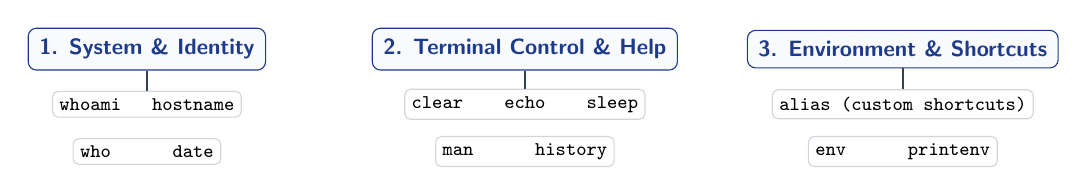
\begin{tikzpicture}[
  x=1cm, y=1cm,
  groupbox/.style={draw=primary, fill=boxbg, rounded corners=3pt, font=\sffamily\footnotesize\bfseries, inner sep=4pt, text=primary},
  cmdbox/.style={draw=bordergray, fill=white, rounded corners=2pt, font=\ttfamily\scriptsize, inner sep=2.5pt}
]
  % Category 1
  \node[groupbox] (g1) at (-4.8, 0) {1. System \& Identity};
  \node[cmdbox] (c1) at (-4.8, -0.7) {whoami \ \ hostname};
  \node[cmdbox] (c2) at (-4.8, -1.3) {who \ \ \ \ \ date};

  % Category 2
  \node[groupbox] (g2) at (0, 0) {2. Terminal Control \& Help};
  \node[cmdbox] (c3) at (0, -0.7) {clear \ \ \ echo \ \ \ sleep};
  \node[cmdbox] (c4) at (0, -1.3) {man \ \ \ \ \ history};

  % Category 3
  \node[groupbox] (g3) at (4.8, 0) {3. Environment \& Shortcuts};
  \node[cmdbox] (c5) at (4.8, -0.7) {alias (custom shortcuts)};
  \node[cmdbox] (c6) at (4.8, -1.3) {env \ \ \ \ \ printenv};

  % Connecting lines
  \draw[-, thick, darkslate] (g1) -- (c1);
  \draw[-, thick, darkslate] (g2) -- (c3);
  \draw[-, thick, darkslate] (g3) -- (c5);
\end{tikzpicture}
\end{center}
\vspace{-8pt}

% =========================================================
% 5. Procedure / Steps
% =========================================================
\section{Procedure / Steps}
We tested the utilities systematically using the following simple steps:
\begin{enumerate}[noitemsep,topsep=1pt,leftmargin=1.4em]
  \item Checked our logged-in identity with \cmd{whoami} and machine hostname with \cmd{hostname}.
  \item Listed active user logins on the terminal with \cmd{who} and printed the system time with \cmd{date}.
  \item Printed a welcome message using \cmd{echo} and tested a timed delay using \cmd{sleep 2}.
  \item Cleared the terminal viewport using the \cmd{clear} command.
  \item Consulted the official manual page for the \cmd{echo} utility using \cmd{man echo}.
  \item Created a convenient command shortcut \cmd{alias ll='ls -lh'} and verified that it works.
  \item Checked exported environment variables such as \cmd{USER} and \cmd{SHELL} using \cmd{printenv} and \cmd{env}.
  \item Reviewed our complete session history using the \cmd{history} command.
\end{enumerate}

% =========================================================
% 6. Result / Output Demonstration (Session 1)
% =========================================================
\section{Result / Output Demonstration}
All commands were executed under user account \texttt{ratul} on host machine \texttt{firefly}.

\subsection{Session 1: Identity, System Time, Output Display, and Documentation}

\terminalwindow{ratul@firefly: \textasciitilde\ \textemdash\ bash}{
% Command 1: hostname & whoami
\termprompt[\textasciitilde]\textbf{\textcolor{termcmd}{hostname \&\& whoami}}

\textcolor{termout}{firefly}

\textcolor{termout}{ratul}

\vspace{0.08cm}
% Command 2: who
\termprompt[\textasciitilde]\textbf{\textcolor{termcmd}{who}}

\textcolor{termout}{ratul\ \ \ \ pts/0\ \ \ \ \ \ \ \ 2026-10-08 09:15 (:0)}

\vspace{0.08cm}
% Command 3: date
\termprompt[\textasciitilde]\textbf{\textcolor{termcmd}{date}}

\textcolor{termout}{Thu Oct  8 10:30:15 UTC 2026}

\vspace{0.08cm}
% Command 4: echo and sleep
\termprompt[\textasciitilde]\textbf{\textcolor{termcmd}{echo "Testing delay..." \&\& sleep 2 \&\& echo "Ready!"}}

\textcolor{termout}{Testing delay...}

\textcolor{termuser}{Ready!}

\vspace{0.08cm}
% Command 5: clear
\termprompt[\textasciitilde]\textbf{\textcolor{termcmd}{clear}}

\textcolor{termhidden}{[Screen cleared successfully]}

\vspace{0.08cm}
% Command 6: man
\termprompt[\textasciitilde]\textbf{\textcolor{termcmd}{man echo | head -n 4}}

\textcolor{termdir}{\textbf{ECHO(1)\ \ \ \ \ \ \ \ \ \ \ \ \ \ \ \ \ \ \ \ \ \ \ \ \ \ \ \ \ \ User Commands\ \ \ \ \ \ \ \ \ \ \ \ \ \ \ \ \ \ \ \ \ \ \ \ \ \ \ \ \ \ ECHO(1)}}

\textcolor{termout}{\textbf{NAME}}

\textcolor{termout}{\ \ \ \ \ \ echo - display a line of text}

\vspace{0.08cm}
% Active cursor
\termprompt[\textasciitilde]\textbf{\textcolor{termcmd}{\rule{0pt}{0.9em}\textunderscore}}
}

\paragraph{Explanation of Session 1 Results:}
\begin{itemize}[noitemsep,topsep=1pt,leftmargin=1.2em]
  \item \cmd{hostname} and \cmd{whoami}: Displayed our computer name (\texttt{firefly}) and user identity (\texttt{ratul}).
  \item \cmd{who}: Showed the active terminal session on pseudoterminal \texttt{pts/0} with login timestamp.
  \item \cmd{date}: Displayed the full current system date, time, and timezone.
  \item \cmd{echo} and \cmd{sleep 2}: \cmd{echo} printed text to stdout, while \cmd{sleep 2} paused execution for 2 seconds.
  \item \cmd{clear} and \cmd{man echo}: \cmd{clear} wiped the terminal view, and \cmd{man echo} provided official documentation.
\end{itemize}

\newpage

% =========================================================
% 6. Result / Output Demonstration (Session 2)
% =========================================================
\subsection{Session 2: Command Shortcuts (Alias), Environment Variables, and History}

\terminalwindow{ratul@firefly: \textasciitilde\ \textemdash\ bash}{
% Command 7: alias
\termprompt[\textasciitilde]\textbf{\textcolor{termcmd}{alias ll="ls -lh"}}

\vspace{0.08cm}
% Command 8: test alias
\termprompt[\textasciitilde]\textbf{\textcolor{termcmd}{ll}}

\textcolor{termout}{total 8.0K}

\textcolor{termperm}{drwxr-xr-x}\ 2\ \textcolor{termuser}{ratul}\ \textcolor{termhost}{users}\ \textcolor{termsize}{\textbf{4.0K}}\ Oct\ \ 8\ 09:30\ \textcolor{termdir}{\textbf{Documents}}

\textcolor{termperm}{-rw-r--r--}\ 1\ \textcolor{termuser}{ratul}\ \textcolor{termhost}{users}\ \textcolor{termsize}{\textbf{1.2K}}\ Oct\ \ 8\ 10:12\ \textcolor{termfile}{notes.txt}

\vspace{0.08cm}
% Command 9: printenv
\termprompt[\textasciitilde]\textbf{\textcolor{termcmd}{printenv USER SHELL}}

\textcolor{termout}{ratul}

\textcolor{termout}{/bin/bash}

\vspace{0.08cm}
% Command 10: env with grep
\termprompt[\textasciitilde]\textbf{\textcolor{termcmd}{env | grep -E "USER|HOSTNAME|HOME"}}

\textcolor{termout}{HOME=/home/ratul}

\textcolor{termout}{HOSTNAME=firefly}

\textcolor{termout}{USER=ratul}

\vspace{0.08cm}
% Command 11: history
\termprompt[\textasciitilde]\textbf{\textcolor{termcmd}{history | tail -n 6}}

\textcolor{termhidden}{\ \ 42\ \ hostname \&\& whoami}

\textcolor{termhidden}{\ \ 43\ \ date}

\textcolor{termhidden}{\ \ 44\ \ echo "Testing delay..." \&\& sleep 2}

\textcolor{termhidden}{\ \ 45\ \ alias ll="ls -lh"}

\textcolor{termhidden}{\ \ 46\ \ printenv USER SHELL}

\textcolor{termhidden}{\ \ 47\ \ history | tail -n 6}

\vspace{0.08cm}
% Final prompt
\termprompt[\textasciitilde]\textbf{\textcolor{termcmd}{\rule{0pt}{0.9em}\textunderscore}}
}

\paragraph{Explanation of Session 2 Results:}
\begin{itemize}[noitemsep,topsep=1pt,leftmargin=1.2em]
  \item \cmd{alias ll="ls -lh"}: Created a custom shortcut named \texttt{ll}. Running \cmd{ll} immediately executed the long listing command with human-readable file sizes.
  \item \cmd{printenv USER SHELL}: Queried the system environment for specific variables, confirming our username and default shell.
  \item \cmd{env | grep ...}: Displayed all global environment variables and filtered for home directory, hostname, and user.
  \item \cmd{history}: Printed the numbered list of previously executed commands, demonstrating how Linux records shell activity so users can recall commands.
\end{itemize}

% =========================================================
% 7. Conclusion
% =========================================================
\section{Conclusion}
In this lab, we practiced everyday command-line utilities that improve terminal productivity in Linux:
\begin{enumerate}[noitemsep,topsep=1pt,leftmargin=1.4em]
  \item We determined active system state, user session, and hardware identity using \cmd{whoami}, \cmd{who}, \cmd{hostname}, and \cmd{date}.
  \item We controlled terminal output and execution timing using \cmd{echo}, \cmd{sleep}, and \cmd{clear}, and accessed documentation with \cmd{man}.
  \item We configured custom command shortcuts using \cmd{alias} to save repetitive keystrokes.
  \item We inspected global configuration settings with \cmd{env} and \cmd{printenv}, and tracked command history with \cmd{history}.
\end{enumerate}
These utilities form the foundation of a comfortable, efficient, and professional Linux command-line workflow.

\end{document}
